\documentclass{article}
\usepackage{amsmath}
\usepackage{graphicx}
\usepackage{listings}
\usepackage{hyperref}
\usepackage{float}
\title{\textbf{Hardware Project - Scientific Calculator}}
\author{P. Shiny Diavajna\\EE24BTECH11058}
\date{\today}

\begin{document}
\maketitle

\section{Introduction}
This report presents the design and implementation of a scientific calculator using the ATmega328P microcontroller and an LCD display. The calculator performs basic arithmetic operations (addition, subtraction, multiplication, division), trigonometric functions (sine, cosine, tangent) and logarithmic functions (log , ln). The primary goal is to implement a versatile and efficient calculator that can display results on an LCD.

\section{Hardware Components}
The following hardware components were used in the project:
\begin{itemize}
    \item Arduino UNO
    \item 16x2 LCD Display
    \item 23 Push Buttons
    \item Resistors (9 15k$\Omega$ ,1 2k$\Omega$, 1 1k$\Omega$,1 1.5 k $\Omega$)
    \item Breadboard
    \item Jumper Wires and connecting wires 
    \item Power Supply 
\end{itemize}

\section{Software and Tools}
The following software and tools were utilized:
\begin{itemize}
    \item AVR GCC Compiler
    \item ArduinoDroid for uploading the HEX file
    \item Termux for file management and HEX file handling
    \item Mathematical Functions (math.h) for trigonometric calculations
    \item LCD Control (util/delay.h) for time management
\end{itemize}


\section{Circuit Design}
\begin{enumerate}
    \item Connect 5V and Ground from the Arduino onto the breadboard.
    \item Connect the push buttons in 2 rows (each from grid to power lines not connected to Ground or 5V). The first row must have 10 buttons (for digits), and the second row must have 13 buttons (for functions). Connect one terminal of each button to Ground.
\end{enumerate}
 
\subsection{Connections}
     \begin{table}[h!]
    \centering
    \begin{tabular}{|c|c|}
        \hline
        \textbf{One end of Jumper Wire}  & \textbf{Another end of Jumper Wire} \\
        \hline
          Digital pin 0 & Push button 16 \\
          Digital pin 1 & Push button 17 \\
          Digital pin 2 & LCD pin 4 \\
          Digital pin 3 & LCD pin 6 \\
          Digital pin 4 & LCD pin 11 \\
          Digital pin 5 & LCD pin 12 \\
          Digital pin 6 & LCD pin 13 \\
          Digital pin 7 & LCD pin 14 \\
          Digital pin 8 & Push button 18 \\
          Digital pin 9 & Push button 19 \\
          Digital pin 10 & Push button 20 \\
          Digital pin 11 & Push button 21 \\
          Digital pin 12 & Push button 22 \\
          Digital pin 13 & Push button 23 \\
          Analog pin A1 & Push button 15 \\
          Analog pin A2 & Push button 14 \\
          Analog pin A3 & Push button 13 \\
          Analog pin A4 & Push button 12 \\
          Analog pin A5 & Push button 11 \\
          Analog pin A0 & Push buttons 1-10 (digit buttons)\\
          LCD pin 1 & Ground \\
          LCD pin 2 & 5V \\
          LCD pin 15 & 5V via 1k $\Omega$ resistor \\
          LCD pin 16 & Ground \\
          LCD pin 3 & Ground via 1.5 k $\Omega$ resistor \\
          LCD pin 5 & Ground \\
          LCD pin 5 & All push buttons \\
          
        \hline
    \end{tabular}
\end{table}

\newpage
\subsection{Push Button Designations}
     \begin{table}[h!]
    \centering
    \begin{tabular}{|c|c|}
        \hline
        \textbf{Button number}  & \textbf{Function} \\
        \hline
           1 - 10 & Digits 0 - 9 \\
           11 & Clear \\
           12 & $\ln{(x)}$ and $\log{(x)}$ \\
           13 & Right Parenthesis \\
           14 & $\sin{(x)}$, $\cos{(x)}$, and $\tan{(x)}$ \\
           15 & $e$ and $\pi$ \\
           16 & Backspace \\
           17 & Decimal Point \\
           18 & Equal To \\
           19 & Left Parenthesis \\
           20 & Division (/)\\
           21 & Multiplications (*)\\
           22 & Subtraction(-) \\
           23 & Addition (+) \\
        \hline
    \end{tabular}
\end{table}


\subsection{Circuit Diagram}
\begin{figure}[H] 
    \centering
    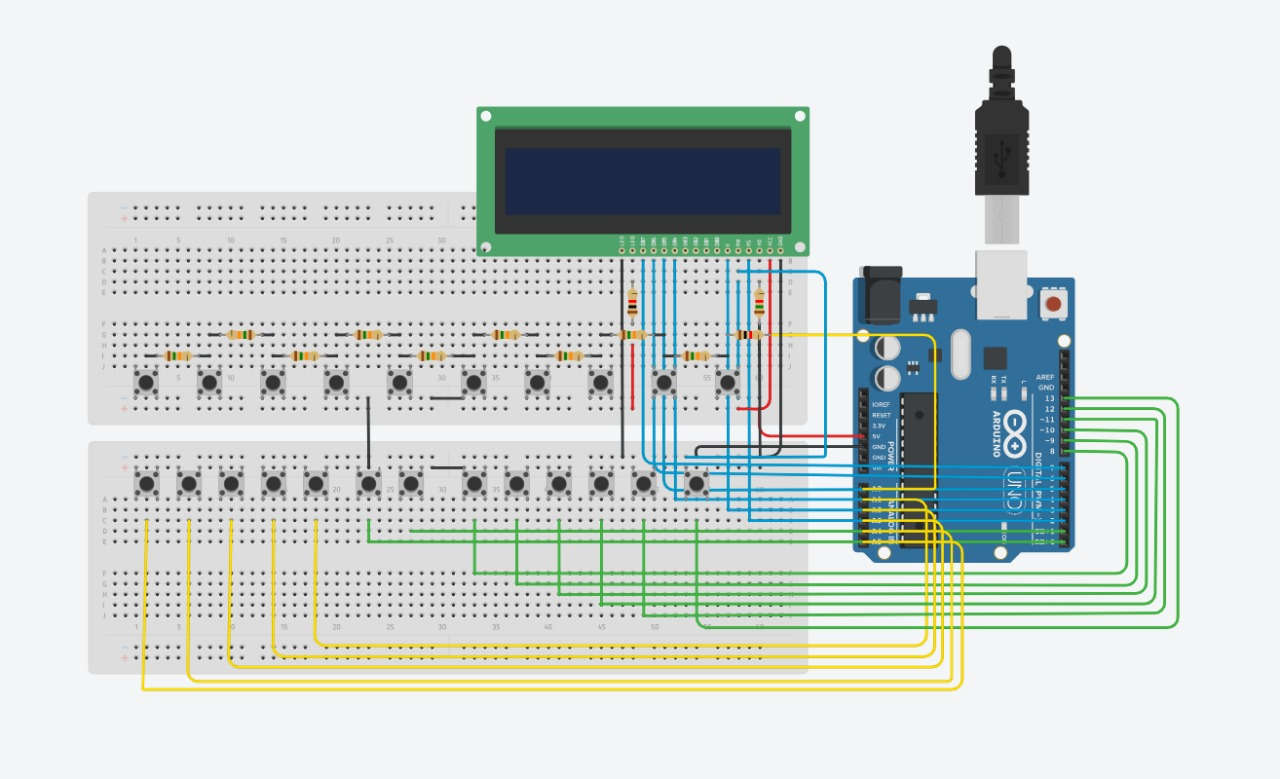
\includegraphics[width=1\textwidth]{Figures/tinkercad.jpeg}
    \caption{Circuit Diagram of the Scientific Calculator}
    \label{fig:circuit}
\end{figure}


  

 

\section{AVR Code}
 The code follows a structured approach:
\begin{itemize}
    \item Initialization of LCD and keypad
    \item Interrupt-based button handling
    \item Mathematical function execution
    \item Displaying results on the LCD
\end{itemize}


 
\section{Results}
The scientific calculator accurately calculates trigonometric functions, basic arithmetic operations and logarithmic functions and displays the results on the LCD display.

 
 
\section{Conclusion}
This project successfully implemented a basic scientific calculator using AVR-GCC and embedded C. The system demonstrates reliable performance in performing calculations while maintaining a simple user interface.\\\\
Acknowlegdement : \\Circuit designed with the help of designed with the help of Akshara EE24BTECH11003, Akshita EE24BTECH11054\\
Code sourced from Akshara EE24BTECH11003, Teja Vardhan EE24BTECH11034, Rasagna EE24BTECH11023, Akhila EE24BTECH11055



\end{document}

